	\chapter{重修线性代数5——空间}
	把线性空间分解成为对其运算封闭的子空间,了解子空间的直和,正交子空间,以及由算子生成的零空间和像空间,这对分析算子,简化计算以及了解结构都是一把犀利的解剖刀。
	
\subsection{子空间}
	
	线性空间是对线性运算封闭的集合。线性空间中的一个子集,如果也对线性运算封闭,即它里面任何几个向量经过线性组合后仍在这子集中,则称为\textbf{线性子空间},在没有歧义的情况简称为\textbf{子空间}。很明显,线性空间本身以及单个零向量都是平凡的子空间。一切子空间都包含着零向量。不要把子空间想象成空间中一个有边缘的几何体,子空间中任何向量的数乘,即任意的延伸都在这子空间里。高于一维的线性空间有无数不同的子空间。在三维空间中,一维的子空间是过原点的一条直线,二维子空间是过原点的一个平面,你以此来推想高维的子空间。
	
	一组向量的线性组合构成了一个子空间,称为这组向量张成的子空间。这子空间的维数,等于这组向量中线性无关向量的个数。一组线性无关的向量,意味着其中任何一个向量都不能在其它几个张成的子空间里,这就像平行六面体的三条棱边不在任何两边确定的平面里。
	
	子空间的交集仍是一个子空间,它们的并集一般则不是,但可用里面向量的线性组合扩充成一个子空间。任取一组向量,它们所有线性组合的集合是个子空间,称为这组向量张成的线性子空间。显然任何一个向量都可以张成一维子空间,k个线性无关的向量张成k维子空间,线性空间中的基张成了整个线性空间。
	
	线性空间中的几个子空间,如果它们相互间除了零向量外没有交集,它们张成的空间,称为这些子空间的直和。直和空间中的向量,都可以用这几个子空间中各有一个向量之和组成,这种分解是唯一的。直和空间里向量运算,等于它分别在子空间里的运算之和。
	
	\kaishu
	
	例如:$ a\begin{pmatrix}1\\2\end{pmatrix},\; b\begin{pmatrix}0\\ 1\end{pmatrix}, \;\; \forall  a,b \in \mathbb{R} $分别都是 $ \mathbb{R}^2 $ 的一维子空间,$ \mathbb{R}^2 $ 是它们的直和。
	
	\songti
	
	分别来自两个子空间中的向量,如果它们的内积都为零,则称这两个子空间是\textbf{正交的}。它们张成的空间是它们的直和。不是全空间或单个零向量的子空间称为\textbf{真子空间}。与真子空间正交的向量构成与它正交的子空间,它们的直和是全空间。
	
	\kaishu
	
	矩阵   $ A=\begin{pmatrix} 1&1&0 \\1&0 &1\end{pmatrix} $  的两个行向量张成  $ \mathbb{R}^3 $ 的二维子空间。方程 $ Ax=0 $ 的所有的解 $ x= a\begin{pmatrix}1&-1&-1 \end{pmatrix}^T,a\in \mathbb{R} $  构成 $ \mathbb{R}^3 $的一维子空间。不难验证$ A $的行向量张成的空间和这方程的解空间是正交的,它们的直和是  $ \mathbb{R}^3 $ 。
	
	\songti
	
	假设线性空间X是子空间W和V的直和,因为向量对子空间直和的分解是唯一的, X中每个向量都对应着子空间W中的一个向量,这个映射称为X对W子空间的\textbf{投影}。空间X中的向量线性运算与它们在W子空间中的投影也保持这种对应,这个性质称为线性空间X与它的子空间W是同态的。\textbf{同态}是在两个代数结构中保持运算不变的映射,对子空间的投影映射是一个同态映射。以前介绍的“同构”,则要求这种映射还是一一满映射。同态映射定义了一种等价关系,它把等价的元素映成同一个像元素,而令其等价的称为同态映射的\textbf{核}。子空间V是X投影到W映射的核,它的投影是零向量,如果X中任何两个向量之差在V中,它们对投影映射则是等价的,投影到W中同一个向量。由此可以进一步学习泛代数的概念,定义在等价关系下的\textbf{商空间},以及商空间与映射像同构关系的基本定理。
	
	\subsection{算子的零空间和像空间}
	
	线性算子保持两个空间的线性运算不变,所以它是一个同态映射。线性算子$  f:X \to Y $ 它的核 $ Ker(f)  $和像$  Im(f) $  定义如下:
	\begin{gather*}
		Ker(f) = \{ x\in X | f(x)= 0 \} ,Im (f) = \{f (x)| x \in X\}  
	\end{gather*}

	$ Ker(f)  $是$  X  $中被$ f $映射为0的向量构成的子空间,也称为算子的零空间。$ X $中两个向量之差如果在零空间中,它可以被线性算子看成是等价的,它们被映到$ Y $中的同一个向量。
	
	而$ Im(f)  $是 $ X $中所有向量被$ f $映射到$ Y $的像构成的子空间,也称为算子的值域。对这些子空间的维数有\textbf{秩-零度定理}:  $ dim(Ker(f))+dim (Im(f))=dim(X) $,它是线性代数的一个基本定理。
	
	\begin{figure}[h]
		\centering
		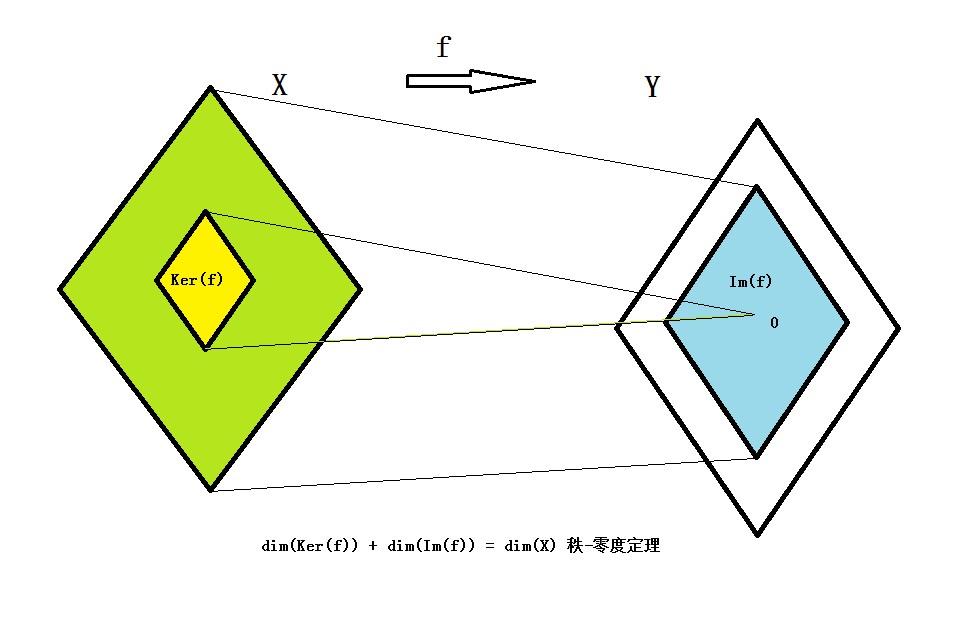
\includegraphics[width=0.7\linewidth]{pic/160449rx8lvzcxlgan88va.png}
		\caption{秩-零度定理}
		\label{fig:160449rx8lvzcxlgan88va}
	\end{figure}
	
	
	维数$  dim(Im(f))  $叫做线性算子f的\textbf{秩},记为 $ rank f $,$ dim(Ker(f)) $叫做线性算子$ f $的\textbf{零度},记为$ nullity f $。满映射的线性算子称为是\textbf{满秩}的,满秩的线性算子的零度为0. 
	
	这个定理似乎很抽象,下面我们从矩阵和方程的角度来看它。
	
	线性算子$ f $将$ X $中的向量$ x $映成$ Y $中的向量,如果存在着$ Y $上的一个线性算子$ f* $,它将$ Y $中的向量$ y $映成$ X $中的向量,使得内积$ \left\langle y, f(x)\right\rangle = \left\langle f*(y), x\right\rangle $,算子$ f* $称为$ f $的\textbf{共轭算子}。不难证明,在实数域算子的矩阵表示中,$ A $的共轭算子是它的转置矩阵$ A^T $(在复数域上是A的共轭转置矩阵$ A* $,为直观起见,我们只介绍实数域的情况,读者自行修正复数域上表示。)
	
	将线性算子$ f $表示为矩阵$ A $,$ A $的列向量张成的子空间称为$ A $的\textbf{列空间},它是算子A的像空间。$ Ax=0 $解构成的子空间称为$ A $的\textbf{右零空间},它是算子$ A $的零空间。
	
	$ A $的行向量张成的子空间称为$ A $的\textbf{行空间},它是共轭算子的列空间。共轭算子$ A^T $的零空间称为$ A $的\textbf{左零空间}。	
	
	齐次线性方程$ Ax=0 $的解构成$ A $的零空间,这方程式说明矩阵的行向量与方程解列向量的内积为零。所以,矩阵的行空间与右零空间总是正交的,它们的直和是矩阵作为线性算子定义域的线性空间。将矩阵转置,对$ A^T $也有相同的结论,即矩阵$ A $的列空间与左零空间也总是正交的,它们的直和是矩阵作为线性算子值域所在的线性空间。矩阵把它的定义域空间X分解为正交的右零空间和行空间的直和,把值域空间分解为正交的左零空间和列空间的直和。试着用内积式子$ \left\langle y, f(x)\right\rangle = \left\langle f*(y), x\right\rangle = 0 $做出上述的解释。
	
	通过矩阵的行和列的操作,可以证明:\textbf{矩阵的行秩等于列秩}。这是线性代数另一个基本定理。我们不再区分矩阵列空间和行空间的维数,统称为矩阵的秩,或算子的秩。
	
	\subsection{线性算子的核与像空间的分解}
	
	联系着算子和共轭算子的子空间分解对理解它们的结构十分重要,这里从矩阵的角度来总结。
	
	表示线性算子的矩阵$ A $,它的核$ Ker(A) $是所有映射成零的向量集合,构成了X中的一个子空间;它的像$ Im(A) $是所有映射得到向量的集合,构成了$ Y $中的一个子空间。算子或矩阵的秩k,是像空间的维数 $ dim(Im(A)) = k $。秩-零度定理说: $ dim(Im(A))+dim(Ker(A)) = dim(X) = n $. 这矩阵的转置$ A^T $表示从$ Y $到$ X $,是与原来对偶的线性算子。同样依秩-零度定理有:$ dim(Im(A^T)) + dim(Ker(A^T)) = dim(Y) = m $. 线性代数的另一个基本定理说:矩阵的行秩等于列秩,即$ dim(Im(A)) = dim(Im(A^T)) = k $,算子与它的对偶算子有相同的秩,所以算子与它的对偶算子的零度分别是:
		$ dim(Ker(A)) = n-k,\quad dim(Ker(A^T)) = m-k $. 
	
	\begin{figure}[h]
		\centering
		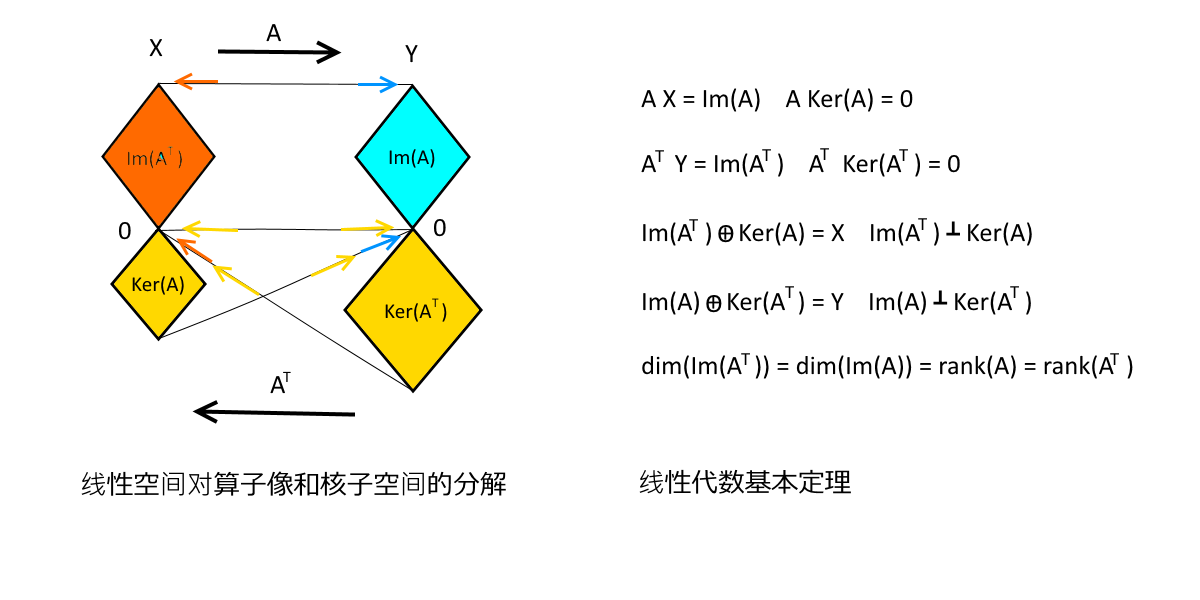
\includegraphics[width=0.7\linewidth]{pic/1604494yzy1do1yro41gva.png}
		\caption{线性代数基本定理}
		\label{1604494yzy1do1yro41gva}
	\end{figure}

	算子$ A $将核空间$ Ker(A) $中的向量映射为零向量,即矩阵中的行向量与它正交,而矩阵中的行向量张成转置矩阵的像空间$ Im(A^T) $。所以线性空间$ X $可以分解成正交的$ k $维子空间$ Im(A^T) $与$ n-k $维子空间$ Ker(A) $的直和,$ Y $可以分解成正交的$ k $维子空间$ Im(A) $与$ m-k $维子空间$ Ker(A^T) $的直和。这意味着$ X $的$ Im(A^T) $子空间中,线性无关向量在$ A $映射下的像也是线性无关的。对$ Y $也有相应的结论。
	\begin{gather*}
		Im(A^T)\oplus Ker(A)=X  Im(A)\oplus Ker(A^T)=Y
	\end{gather*}
	
	\subsection{线性空间和算子的不变量}
	
	线性空间的特征是\textbf{维数},它是空间中线性无关向量的最大个数,无论空间中的元素是什么具体的数学实体,同一维数的线性空间都对线性运算同构,都可以用相同维数坐标的列向量来表示。
	
	算子的\textbf{秩}是象空间的维数。$ n $维到$ m $维线性空间上的线性算子,在给定基的坐标下表示为一个$ m*n $矩阵。算子的象空间对应着矩阵列向量所张成的线性子空间,所以矩阵的秩等于它列向量中最大线性无关的个数。
	
	改变映射两边线性空间的基,表示线性算子的矩阵也随之改变。它们是同一个线性算子的不同表示,所以这些矩阵的秩都是一样的,秩是在基的变动中,矩阵表示保持不变的固有性质。
	
	空间中不同基之间对应着一个线性变换满映射,将一组基映射成另一组基,它可以表示为一个满秩的方阵。反之,满秩的方阵对应着两组基坐标间的变换。相同秩的$ m*n $矩阵,总是可以通过左右两边各乘以一个满秩的方阵变成一样。所以它们是同一个线性算子在不同基坐标下的矩阵表示。秩是$ m*n $矩阵在坐标变换中的不变量,它们对应着同一个线性算子。
	
	\subsection{无穷维线性空间}
	
	可以找到任意多个线性无关向量的线性空间,称为\textbf{无穷维线性空间},例如多项式空间,解析函数空间等等。我们知道所有解析函数都可以展开成泰勒级数,即等于无穷多个基向量的线性组合,是不是所有无穷维线性空间都能如此?
	
	大致是如此,但无穷多个基不一定都是可数的,也可能是连续谱的,其线性组合不限于无穷级数形式的和,还可能是积分形式的和。无穷多项的线性组合的含义,涉及到收敛和完备性的概念,这依赖于空间中的拓扑结构。
	
	代数只关心集合中元素运算的性质,而不涉及集合中元素的“相邻”和“远近”,这后者是拓扑关系,需在集合中另行定义。所以通常线性代数的课程只介绍有限维空间的向量和算子,这不需要了解空间拓扑的性质。但它的内容同样适用于无穷维的空间,只是涉及到向量“无穷和”时,需要收敛的概念。无穷维线性空间的内容多在泛函分析中介绍。
	
	我们脑中对向量想象的图像,通常是三维的几何空间,这是在实数域上以向量的内积赋予长度的概念,从而有可以度量远近的欧几里德空间。抽象的线性空间未必如此,所以我们以直观的图像想象抽象世界时,必须清醒地认识这些不同,头脑中“看到”的结果必须从定义出发用严谨的逻辑推理来验证它。
	
	在加法和数乘下封闭的一族函数集合是个线性空间,可以定义不同的“距离”,就有不同的收敛,例如点点收敛,一致收敛,几乎处处收敛等等。收敛性保证这无穷线性组合的分解有意义,完备性是说任何这类无穷线性组合的向量仍在这线性空间中。对此有兴趣可以看我“重修微积分”系列的博文。
	
	在无穷维线性空间中应用最多的是用内积定义距离完备的线性空间,称为\textbf{希尔伯特空间}。函数表示为傅立叶级数,贝塞尔函数级数等特殊函数都是在线性空间基上的分解。因为微分算子是线性的,在物理中许多微分方程都可以看成一个线性系统,而线性系统可以用叠加原理,当方程的解可以表示为一个函数族基向量的线性组合,微分算子作用在这些函数上仍然是它们的线性组合,微分方程以此化为代数方程组。这是在计算机时代前,历史上为微分方程的解法,发展出物理图像解释的数学根据。